%%%%%%%%%%%%%%%%%%%%%%%%%%%%%%%%%%%%%%%%%%%%%%%%%%%%%%%%%%%%%%%%%%%%%%%%%%%%%%%%
%%  Sample document for preparing papers to  "Avtomatika i Telemekhanika"
%%  charset=utf-8
%%%%%%%%%%%%%%%%%%%%%%%%%%%%%%%%%%%%%%%%%%%%%%%%%%%%%%%%%%%%%%%%%%%%%%%%%%%%%%%%

\documentclass[12pt]{a&t}
\usepackage{graphicx}
\usepackage{caption}
\usepackage{bm}
\usepackage{url}
\usepackage{multirow}
\usepackage{cmap}
\usepackage{autonum}
\usepackage{cite}

\usepackage[labelformat=empty]{caption}
% \renewcommand{\baselinestretch}{2}

\begin{document}

\year{2022}

\title{АНАЛИЗ СВОЙСТВ ВЕРОЯТНОСТНЫХ МОДЕЛЕЙ В ЗАДАЧАХ ОБУЧЕНИЯ С ЭКСПЕРТОМ}%
\thanks{Исследование выполнено при финансовой поддержке Российского фонда фундаментальных исследований в рамках научных проектов 20-37-90050, 19-07-01155 и проекта Национальной технологической инициативы 13/1251/2018.}


\authors{А.И.~БАЗАРОВА (bazarova.ai@phystech.edu),\\
А.В.~ГРАБОВОЙ (grabovoy.av@phystech.edu)\\
(Московский физико-технический институт),\\
В.В.~СТРИЖОВ, д-р~физ.-мат.~наук (strijov@phystech.edu)\\
(Вычислительный центр им. А.А. Дородницына ФИЦ ИУ РАН)}

\maketitle

\begin{abstract}
Работа посвящена построению интерпретируемых моделей машинного обучения.
Решается задача аппроксимации набора фигур на контурном изображении.
Вводятся предположения, что фигуры являются кривыми второго порядка.
При аппроксимации фигур используются информация о типе, расположении и форме кривых, а также о множестве их возможных преобразований.
Такая информация называется \textit{экспертной}, а метод машинного обучения, основанный на экспертной информации, называется \textit{обучение с экспертом}.
Предполагается, что набор фигур аппроксимируется набором \textit{локальных моделей}.
Каждая локальная модель, основанная на экспертной информации, аппроксимирует одну фигуру на контурном изображении.
Для построения моделей предлагается отображать кривые второго порядка в пространство признаков, в котором каждая локальная модель является линейной.
Таким образом, кривые второго порядка аппроксимируются набором линейных моделей.
В вычислительном эксперименте рассматривается задача аппроксимации радужной оболочки глаза на контурном изображении.

\smallskip\\
\textit{Ключевые слова}: смесь экспертов; экспертное обучение; линейные модели; интерпретируемые модели.
\end{abstract}

\section{Введение}
Современные решения задачи классификации изображений на основе сетей глубокого обучения ResNet, VGG, Intercept~\cite{Kaiming2015} представляют собой плохо интерпретируемые модели~\cite{Ribeiro2016}.
В~\cite{Han2020, Akhtar2018} показано, что сети глубокого обучения являются не устойчивыми даже к небольшому шуму в данных~\cite{Grabovoy2022ait}.

В данной работе предлагается метод \textit{обучения с экспертом}.
Метод предполагает использование экспертной информации для повышения качества аппроксимации, а также для получения интерпретируемых моделей машинного обучения.
Предметные знания экспертов о данных называются~\textit{экспертная информация}.
Предполагается, что использование экспертной информации позволяет аппроксимировать выборку простыми интерпретируемыми моделями, такими как линейные модели. Метод машинного обучения, учитывающий экспертные знания при построении моделей, называется~\textit{обучение с экспертом}.
В данной работе решается задача аппроксимации кривых второго порядка на контурном изображении.
В работе анализируются кривые второго порядка, так как они описываются линейными моделями. Параметры кривых второго порядка необходимо восстановить в задаче распознавания радужной оболочки глаза~\cite{Matveev2010, Matveev2014, Bowyer2010}, в задаче описания трека частицы в адронном коллайдере~\cite{Dalila2018}.
Экспертная информация о кривой второго порядка отображает точки на плоскости в новое признаковое описание объекта. 
Каждая кривая аппроксимируется одной линейной моделью.
Модель, аппроксимирующая кривую, называется \textit{локальной моделью}.
Для аппроксимации всего контурного изображения требуется аппроксимация нескольких кривых второго порядка с использованием локальных моделей.
Вводятся следующие ограничения на изображения: а) изображение состоит только из кривых второго порядка; б) изображение аппроксимируется небольшим числом кривых второго порядка; в) известно число и тип кривых на изображении.\marginpar{Рис. \ref{intro:fig2}.}

На рис.~\ref{intro:fig2} показан пример кривых второго порядка, а также экспертная информация о кривых. Рассматривается пример двух кривых, которые задаются своим цветом. На центральном изображении показаны точки, лежащие на кривых, а на рисунках справа и слева представлены экспертные признаковые описания рассмотенных кривых. В каждом из экспертных признаковых описаний получаем, что одна из кривых аппроксимируется линейной моделью, а вторая является шумом относительно построенной линейной модели. Отображение~$K_x^1\bigr(\mathbf{c}\bigr), K_x^2\bigr(\mathbf{c}\bigr), K_y^1\bigr(\mathbf{c}\bigr), K_y^2\bigr(\mathbf{c}\bigr)$ описывается на основе экспертной информации. На рис.~\ref{intro:fig2} слева показана экспертная информация о первом эксперте. С использованием этой информации первая кривая аппроксимируется линейной моделью, а вторая кривая представляет собой шум. На рис.~\ref{intro:fig2} справа показана экспертная информация второго эксперта. С использованием этой информации вторая кривая аппроксимируется линейной моделью, а первая кривая представляет собой шум.

При аппроксимации нескольких кривых на одном контурном изображении строится мультимодель. Примером мультимоделей является случайный лес~\cite{Ishwaran2012}, бустинг деревьев~\cite{Tianqi2016}, смесь экспертов~\cite{Yuksel2012}.
В данной работе в качестве мультимодели рассматривается смесь экспертов.
Смесь экспертов~--- это мультимодель, которая линейно взвешивает локальные модели, аппроксимирующие часть выборки.
Значения весовых коэффициентов зависят от объекта, для которого делается прогноз.
Для решения задачи используется вариационный EM--алгоритм~\cite{Dempster1977, Ebrahimpour2009, Peng1996, Grabovoy2021}.
Смесь экспертов имеет множество применений в ряде приложений.
В~\cite{Estabrooks2001} решается задача классификации текстов.
В~\cite{Cheung1995, Weigend2000, Cao2003, Mossavat2010, Sminchisescu2007, Tuerk2001, Yumlu2003} смесь экспертов используется для прогнозирования временных рядов, для распознавания речи, распознавания повседневной деятельности человека и прогнозирования стоимости ценных бумаг.
В~\cite{Ebrahimpour2009} рассматривалась смесь экспертов для решения задачи распознавания рукописных цифр на изображениях.

В качестве примера рассматривается задача аппроксимации изображения радужной оболочки глаза. На рис.~\ref{intro:fig1} показан пример изображения, которое необходимо аппроксимировать.
В данной работе рассматривается обработанное изображение в виде контурного изображения.\marginpar{Рис. \ref{intro:fig1}.}

Для задачи аппроксимации радужной оболочки используется экспертная информация: радужная оболочка глаза аппроксимируется двумя концентрическими окружностями.
Экспертная информация используется для построения описания признаков точек плоскости, а также для построения регуляризатора в функции оптимизации.
Часть функции ошибок для оптимизации, использующая экспертную информацию, называется регуляризатором.
Таким образом, информация о том, что изображение является окружностями, задается видом признакового описания, а информация о том, что окружности концентрические, задается с помощью специального регуляризатора.

Вычислительный эксперимент анализирует качество аппроксимации контурного изображения в зависимости от экспертной информации и уровня шума в синтетически сформированных данных. Проведен анализ качества аппроксимации радужной оболочки в зависимости от объема экспертной информации, которая использовалась для построения модели.
Каждое аппроксимированное изображение представляет собой отдельный набор точек, которые необходимо аппроксимировать.

\section{Постановка задачи восстановления параметров кривых второго порядка на изображении}
Задано бинарное изображение
\begin{gather}
\mathbf{M} \in \{0, 1 \}^{m_1\times m_2},
\end{gather}
где~$1$ соответствует черной точке изображения, а~$0$ соответствует белой точке фона.
С использованием изображения~$\mathbf{M}$ строится выборка~$\mathbf{C}$, элементами которой являются координаты~$(x_i, y_i)$ черных точек:
\begin{gather}
\mathbf{C} \in \mathbb{R}^{N \times 2}.
\end{gather}
Каждый эксперт предполагает, что изображение состоит из кривой второго порядка~$\Omega$.
Пусть для множества точек~$\mathbf {C} \in \mathbb{R}^{N \times 2} $, образующих кривую $\Omega,$ задана экспертная информация о фигуре $E(\Omega)$.
Множество $E(\Omega)$ состоит из ожидаемого экспертом образа~$\Omega$ и множества его допустимых преобразований. На основе экспертного описания введем отображения в задачу аппроксимации:
\begin{gather}
\label{eq1}
	K_{x}\bigl(E(\Omega)\bigr): \mathbb{R}^{2} \rightarrow \mathbb{R}^{n}, \quad K_{y}\bigl(E(\Omega)\bigr): \mathbb{R}^{2} \rightarrow \mathbb{R},
\end{gather} 
где~$K_{x}$~--- отображение объектов в признаковое описание объектов,~$n$~--- число признаков, а ~$K_{y}$~---  отображение в целевую переменную для аппроксимации. Применяя отображения~$K_{x}, K_{y}$ для выборки~$\mathbf{C}$ поэлементно, получаем:
\begin{gather}
\label{eq2}
	K_{x}\bigl(E(\Omega\bigr), \mathbf{c}) = \mathbf{x}, \quad  K_{y}\bigl(E(\Omega), \mathbf{c}\bigr) = y,
\end{gather}
где~$\mathbf{c} = (x_i, y_i)$~--- точка из множества точек $\mathbf{C}$.

Применяя отображения~\eqref{eq2} к исходному множеству точек~$\mathbf{C}$, получаем выборку
\begin{gather}
\label{eq4}
    \mathfrak{D} = \{(\mathbf{x}, y) \; | \; \forall \mathbf{c} \in \mathbf{C} \; \mathbf{x} = K_x(\mathbf{c}), \; y = K_y(\mathbf{c}) \}.
\end{gather}

Получаем, что исходная задача аппроксимации кривой~$\Omega$ сводится к аппроксимации выборки~$\mathfrak{D}$. В работе предполагается, что выборка~$\mathfrak{D}$ аппроксимируется линейной моделью:

\begin{gather}
	g(\mathbf{x}, \mathbf{w}) = \mathbf{x}^\mathsf{T} \mathbf{w},
\end{gather} 
где~$\mathbf{w}$~--- вектор параметров для аппроксимации.

Для нахождения оптимального вектора параметров~$\hat{\mathbf {w}}$ решается оптимизационная задача
\begin{gather}
	\hat{\mathbf{w}} = \arg\min_{\mathbf{w}\in\mathbb{R}^n} \sum_{\left(\mathbf{x}, y\right) \in \mathfrak{D}}\|g(\mathbf{x}, \mathbf{w}) - y \|_2^2.
\end{gather} 

Задача аппроксимации исходной кривой~$\Omega$ сводится к решению задачи линейной регрессии, т.е. к нахождению компонент вектора $\hat{\mathbf{w}}$.

В случае, когда на изображении~$K$ кривых второго порядка~$\Omega_1, \dots, \Omega_K$, где для каждой задана экспертная информация~$E_k = E(\Omega_k), \, k \in \{1, \dots, K\}$ получаем задачу построения мультимодели, которая называется смесью~$K$ экспертов.

\begin{definition}
Назовем мультимодель~$f$ смесью~$K$ экспертов
\begin{gather}
	f = \sum\limits_{k = 1}^{K}\pi_k(\mathbf{x}, \mathbf{V})g_k(\mathbf{w}_k),  \quad \pi_k(\mathbf{x}, \mathbf{V}): \mathbb{R}^{n\times |\mathbf{V}|} \rightarrow [0, \, 1], \quad \sum\limits_{k = 1}^{K}\pi_k(\mathbf{x}, \mathbf{V}) = 1, 
\end{gather}
где~$g_k$~--- локальная модель, называемая экспертом. Вектор~$\mathbf{x}$~--- признаковое описание объекта, $\pi_k$~--- шлюзовая функция, вектор $\mathbf{w}_k$~--- параметры локальной модели, $\mathbf{V}$ являются параметрами шлюзовой функции.
\end{definition}

Для каждой кривой второго порядка~$\Omega_k$ заданы отображения~\eqref{eq1}. Введем обозначения: $K_x^k\bigr(\mathbf{c}\bigr) = K_x\bigr(\Omega_k, \mathbf{c}\bigr)$ и $K_y^k\bigr(\mathbf{c}\bigr) = K_y\bigr(\Omega_k, \mathbf{c}\bigr)$. Используя локальные линейные модели~$g_k$, строим мультимодель~$f$, описывающую кривые $\Omega_1, \dots, \Omega_K$ на изображении $\mathbf{M}$:
\begin{gather}
\label{5}
	f = \sum\limits_{\mathbf{c} \in \mathbf{C}} \sum_{k = 1}^{K} \pi_k(\mathbf{c}, \mathbf{V})g_k(K^k_{x}\bigl(\mathbf{c}), \mathbf{w}_k), 
\end{gather}
где~$\pi_k$~--- шлюзовая функция. В работе рассматривается случай, когда~$\mathbf{x}=K^1_{x}\bigl(\mathbf{c})=\cdots=K^K_{x}\bigl(\mathbf{ c}).$ В этом случае выражение~\eqref{5} переписывается в виде
\begin{gather}
\label{5_1}
	f = \sum\limits_{\mathbf{c} \in \mathbf{C}} \sum_{k = 1}^{K} \pi_k(\mathbf{x}, \mathbf{V})g_k(\mathbf{x}, \mathbf{w}_k), 
\end{gather}
где шлюзовая функция~$\pi_k$ имеет вид
\begin{gather}
\label{6}
	\pi_k(\mathbf{x}, \mathbf{V}): \mathbb{R}^{n\times |\mathbf{V}|} \rightarrow [0, \, 1], \; \; \; \; \sum\limits_{k = 1}^{K}\pi_k(\mathbf{x}, \mathbf{V}) = 1,
\end{gather}
где~$\mathbf{V}$~--- параметры функции шлюза, а $g_k$~--- локальная модель.

В работе рассматривается следующий вид шлюзовой функции:
\begin{gather}
    \boldsymbol{\pi}(\mathbf{x}, \mathbf{V}) = \text{softmax}\bigl(\mathbf{V}_1^{\mathsf{T}}\boldsymbol{\sigma}(\mathbf{V}_2^{\mathsf{T}}\mathbf{x}) \bigr),
\end{gather}
где~$\mathbf{V} = \{\mathbf{V}_1, \, \mathbf{V}_2\}$~--- параметры шлюзовой функции, $\mathbf{V}_1 \in \mathbb{R}^{p \times k}, \, \mathbf{V}_2 \in \mathbb{R}^{n \times p}$.

Для нахождения оптимальных параметров мультимодели решается оптимизационная задача
\begin{gather}
\label{9}
\mathcal{L} = \sum\limits_{(\mathbf{x}, y) \in \mathfrak{D}} \sum\limits_{k = 1}^{K} \pi_k(\mathbf{x}, \mathbf{V})(y - \mathbf{w}_k^{\mathsf{T}}\mathbf{x})^2 + R\bigl(\mathbf{V}, \mathbf{W}, E(\Omega)\bigr) \rightarrow \min_{\mathbf{V}, \mathbf{W}},
\end{gather}
где~$\mathbf{W} = [\mathbf{w}_1, \dots, \mathbf{w}_k]$~--- параметры локальных моделей, $R\bigl(\mathbf{V}, \mathbf{W}, E(\Omega)\bigr)$~--- параметры регуляризации, основанные на экспертной информации.

\section{Построение признакового описания фигур}
\paragraph{Единое пространство для кривых второго порядка.} Произвольная кривая второго порядка, главная ось которой не параллельна оси ординат, задается  уравнением
\[
\label{st:coef}
x^2 = B'xy+C'y^2+D'x+E'y+F',
\]
где на коэффициенты $B', C'$ накладываются ограничения, зависящие от типа кривой. Выражение~\eqref{eq2} для кривой второго порядка принимает вид
\[
\label{st:K_map}
K_x\bigr(\mathbf{c}_i\bigr)=\left[x_iy_i, y_i^2, x_i, y_i, 1\right], \quad K_y\bigr(\mathbf{c}_i\bigr)=x_i^2,
\]
откуда получаем задачу линейной регрессии для восстановления параметров ~$B', C', D', E', F'$ по заданой выборке.

\paragraph{Окружность.} В качестве частного случая кривой второго порядка рассмотривается окружность.
Пусть~$(x_0, y_0)$~--- центр окружности, которую требуется восстановить на бинарном изображении~$\mathbf{M}$, а $r$~--- ее радиус.
Элементы выборки~$(x_i, y_i) \in \mathbf{C}$ представляют собой геометрическое место точек, которое аппроксимируется уравнением окружности:
\begin{gather}(2x_0) x_i + (2y_0) y_i + (r^2 - x_0^2 - y_0^2) = x_i^2 + y_i^2. 
\end{gather}
Тогда выражение~\eqref{eq2} принимает следующий вид:
\begin{gather}
\label{10}
K_{x}(\mathbf{c}_i) = [x_i, \, y_i, \, 1] = \mathbf{x}, \,  K_{y}(\mathbf{c}_i) = x_i^2+y_i^2 = y.
\end{gather} 
Получаем задачу линейной регрессии~\eqref{eq4}.
Компоненты вектора~$\mathbf{w} = [w_0, \, w_1, \, w_2]^\mathsf{T}$ восстанавливают параметры окружности:
\begin{gather}
x_0 = \frac{w_0}{2}, \; y_0 = \frac{w_1}{2}, \; r = \sqrt{w_3 + x_0^2 + y_0 ^2}.
\end{gather}

\section{Композиция фигур}
Для построения композиции фигур используется уравнение~\eqref{9}, которое принимает вид
\begin{gather} 
\label{statment:optim:task}
\begin{aligned}
\mathcal{L} = \sum\limits_{\mathbf{c} \in \mathbf{C}} \sum\limits_{k = 1}^{K} \pi_k(\mathbf{c}, \mathbf{V})\left(K^{k}_y\bigr(\mathbf{c}\bigr) - \mathbf{w}_k^{\mathsf{T}}K^{k}_x\bigr(\mathbf{c}\bigr)\right)^2 + R\bigl(\mathbf{V}, \mathbf{W}, E(\Omega)\bigr) \rightarrow \min_{\mathbf{V}, \mathbf{W}},
\end{aligned}
\end{gather}
где~$K^{k}_x, K^{k}_y$~--- экспертное представление~$k$-го эксперта. Предполагая, что все кривые на изображении описываются одним признаковым описанием~$\mathbf{x} =K^{1}_x\bigr(\mathbf{c}\bigr)=\cdots=K^{K}_x\bigr( \mathbf{c}\bigr), x= K^{1}_y\bigr(\mathbf{c}\bigr)=\cdots=K^{K}_y\bigr(\mathbf{c}\bigr),$ получаем оптимизационную задачу:
\begin{gather} 
\label{statment:optim:task:simp}
\begin{aligned}
\mathcal{L} = \sum\limits_{\left(\mathbf{x}, y\right) \in \mathfrak{D}} \sum\limits_{k = 1}^{K} \pi_k(\mathbf{x}, \mathbf{V})\left(y - \mathbf{w}_k^{\mathsf{T}}\mathbf{x}\right)^2 + R\bigl(\mathbf{V}, \mathbf{W}, E(\Omega)\bigr) \rightarrow \min_{\mathbf{V}, \mathbf{W}},
\end{aligned}
\end{gather}
где регуляризатор~$R$ учитывает дополнительные ограничения параметров локальных моделей. Для решения задачи оптимизации~\eqref{statment:optim:task:simp} используется EM--алгоритм, описанный в~\cite{Grabovoy2021}.

\section{Вычислительный эксперимент}

Проведен вычислительный эксперимент по анализу качества аппроксимации кривых второго порядка на изображении. Эксперимент разделен на несколько частей. Первая часть описывает эксперимент с несколькими окружностями на изображении. Во второй части анализируется сходимость метода в зависимости от уровня шума в данных и от заданной экспертной информации. В третьей части проводится эксперимент по аппроксимации радужной оболочки глаза.\marginpar{Рис. \ref{ce:fig3}.}

\subsection{Эксперимент по восстановлению параметров окружности}

В этой части эксперимента анализируется аппроксимация нескольких кривых второго порядка предложенной мультимоделью. Аппроксимируется сгенерированная синтетическая выборка. Выборка состоит из трех произвольных непересекающихся окружностей. К окружностям добавлен шум. Шум добавлялся к каждой точке окружности в отдельности, а также в выборку добавлялись случайные точки, не относящиеся к окружности.

На рис.~\ref{ce:fig3} показан результат построения ансамбля локальных аппроксимирующих моделей. Каждая локальная модель аппроксимирует одну окружность. Видно, что при добавлении шума качество аппроксимации падает.
На рис.~\ref{ce:fig4} показан график зависимости радиуса окружностей~$r$ и их центров~$(x_0, y_0)$ от номера итерации.\marginpar{Рис. \ref{ce:fig4}.}

\subsection{Анализ качества аппроксимации для выборки с разным уровнем шума}

В этой части эксперимента анализируется качество аппроксимации~$S$ в зависимости от уровня шума~$\beta$ в данных и от параметра априорных распределений~$\gamma$. Выборка сгенерирована в таком виде: сначала случайным образом выбираются два вектора параметров~$\mathbf{w}^\text{true}_{1}$ и~$\mathbf{w}^\text{true}_{2}$~--- коэффициенты двух парабол. Векторы~$\mathbf {w}^\text {true}_{1}$ и~$\mathbf{w}^\text {true}_{2}$ используются для генерации точек~$x_i$ и~$y_i$ с добавлением нормального шума~$\varepsilon\sim\mathcal {N} \bigr(0,\beta\bigr)$.
При обучении мультимодели учитывается априорное распределение параметров~$\mathbf{w}_1\sim\mathcal{N}\bigr(\mathbf{w}^\text{true}_{1}, \gamma \mathbf{I}\bigr),\mathbf{w}_2\sim\mathcal{N}\bigr(\mathbf{w}^\text{true}_{2}, \gamma\mathbf{I}\bigr)$.

Рассматривается критерий качества:
\[
S = ||\mathbf{w}^\text{pred}_{1} - \mathbf{w}^\text{true}_{1}||^{2}_{2} + ||\mathbf{w}^\text{pred}_{2} - \mathbf{w}^\text{true}_{2}||^{2}_{2},
\]
где~$\mathbf{w}^\text{pred}_{1}$~--- аппроксимация вектора параметров первой локальной модели, а~$\mathbf{w}^\text{pred}_{2}$~--- аппроксимация вектора параметров второй локальной модели.

На рис.~\ref{ce:fig5} показана зависимость критерия качества~$S$ от уровня шума~$\beta$ и параметра априорного распределения~$\gamma$.\marginpar{Рис. \ref{ce:fig5}.} Из графика видно, что при малом уровне шума~$\beta$ качество аппроксимации не зависит от параметра~$\gamma$, а при увеличении шума~$\beta$ качество аппроксимации~$ S$ уменьшается.

На рис.~\ref{ce:fig6} показан пример работы алгоритма с разными параметрами~$\beta$ и $\gamma$.\marginpar{Рис. \ref{ce:fig6}.} Видно, что в отсутствие шума~$\beta$ обе локальные модели аппроксимируют выборку корректно. С ростом уровня шума качество аппроксимации падает: при~$\beta = 0 {,}2$ с ростом $\gamma$ первая локальная модель из параболы преобразовывается в эллипс; для~$\beta=0 {,}4$ с ростом $\gamma$ первая локальная модель из параболы преобразовывается в эллипс, а вторая модель~--- из параболы в гиперболу.

\subsection{Аппроксимация радужки глаза}
Анализ качества аппроксимации проводится для задачи аппроксимации радужной оболочки глаза на изображении. Радужная оболочка глаза состоит из двух концентрических окружностей, поэтому рассматривается мультимодель, состоящая из двух экспертов: каждый эксперт аппроксимирует одну из окружностей. В вычислительном эксперименте сравнивается качество аппроксимации окружностей в случае задания разных регуляризаторов $R_0, R_1, R_2$. Регуляризатор $R_0\bigl(\mathbf{V}, \mathbf{W}, E(\Omega)\bigr)=0,$ что соответсвует отсутсвию регуляризатора. Регуляризатор
\[
R_1\bigl(\mathbf{V}, \mathbf{W}, E(\Omega)\bigr)= -\sum_{k=1}^{K}\mathbf{w}_k^{\mathsf{T}}\mathbf{w}_k
\]
способствует околонулевым параметрам локальных моделей.
Регуляризатор
\[
R_2\bigl(\mathbf{V}, \mathbf{W}, E(\Omega)\bigr)= -\sum_{k=1}^{K}\mathbf{w}_k^{\mathsf{T}}\mathbf{w}_k + \sum_{k=1}^{K}\sum_{k'=1}^{K}\sum_{j=1}^2\left(w_k^j-w_k'^j\right)^2
\]
способствует совпадению центров окружностей и близким к нулю параметрам локальных моделей.

\marginpar{Рис. \ref{ce:fig6-1}.}Рис.~\ref{ce:fig6-1} показывает результат аппроксимации радужной оболочки глаза после~$10$ итераций. Видно, что при отсутствии регуляризатора одна из окружностей находится некорректно.\marginpar{Рис. \ref{ce:fig7}.} В случае задания регуляризатора~$R_1$ модель аппроксимирует обе окружности, но окружности неконцентричны. В случае задания регуляризатора~$R_2$ получаем концентрические окружности на изображении.\marginpar{Рис. \ref{ce:fig8}.}

На рис.~\ref{ce:fig7}--\ref{ce:fig9} показан процесс сходимости мультимоделей в случае указания разных регуляризаторов~$R_0, R_1, R_2$.\marginpar{Рис. \ref{ce:fig9}.} Видно, что модели с регуляризатором типа~$R_1$ и~$R_2$ аппроксимируют обе окружности, а мультимодель с регуляризатором $R_0$ аппроксимирует только большую окружность.

\section{Заключение}
В статье предлагается метод построения интерпретируемых моделей машинного обучения на основе экспертной информации. В качестве задачи рассматривается задача аппроксимации кривых второго порядка: параболы, гиперболы, эллипса. Аппроксимация кривых второго порядка применяется в задаче об аппроксимации радужной оболочки.

Проведен эксперимент, в ходе которого анализируется качество аппроксимации кривых второго порядка в зависимости от начального уровня шума в данных, а также в зависимости от регуляризатора функции ошибки. В ходе эксперимента показано, что с увеличением уровня шума в исходных данных точность аппроксимации снижается: при большом шуме форма аппроксимируемой фигуры меняется с параболы на гиперболу. Проведен вычислительный эксперимент по аппроксимации радужной оболочки глаза двумя концентрическими окружностями. Эксперимент показывает, что регуляризация на основе экспертной информации улучшает качество аппроксимации.

\begin{thebibliography}{}
\bibitem{Kaiming2015}
	\textit{He K., Ren S., Sun J., Zhang X.} Deep Residual Learning for Image Recognition // Proc. IEEE Conf. on Computer Vision and Pattern Recognition. Las Vegas. 2016. P.~770--778.
\bibitem{Ribeiro2016}
	\textit{Ribeiro M., Singh S., Guestrin C.} Why Should I Trust You?: Explaining the Predictions of Any Classifier // Proc. of the 22nd ACM SIGKDD International Conference on Knowledge Discovery and Data Mining. 2016. P.~1135--1144.
\bibitem{Han2020}
	\textit{Han X., Yao M., Debayan D., Hui L., Ji-Liang T., Anil J.} Adversarial Attacks and Defenses in Images, Graphs and Text: A Review // Int. J. Automat. Comput. 2020. V.~17. P.~151--178.
\bibitem{Akhtar2018}
	\textit{Akhtar N., Mian A.} Threat of Adversarial Attacks on Deep Learning in Computer Vision: A Survey // IEEE Access. 2018. V.~6. P.~14410--14430.
\bibitem{Grabovoy2022ait}
	\textit{Grabovoy A., Strijov V.} Probabilistic Interpretation of the Distillation Problem // Autom. Remote Control. 2022. V.~83. P.~123--137.
\bibitem{Matveev2010}
	\textit{Matveev I.} Detection of iris in image by interrelated maxima of brightness gradient projections // Appl. Comput. Math. 2010. V.~9. P.~252--257.
\bibitem{Matveev2014}
	\textit{Matveev I., Simonenko I.} Detecting precise iris boundaries by circular shortest path method // Pattern Recognition and Image Analysis. 2014. V.~24. P.~304--309.
\bibitem{Bowyer2010}
	\textit{Bowyer K., Hollingsworth K., Flynn P.} A Survey of Iris Biometrics Research: 2008-2010 // Handbook of iris recognition. 2010. P.~15--54.
\bibitem{Dalila2018}
	\textit{Salamani D., Gadatsch S., Golling T.,  Stewart G., Ghosh A.,  Rousseau D.,  Hasib A.,  Schaarschmidt J.} Deep Generative Models for Fast Shower Simulation in ATLAS // IEEE 14th International Conference on e-Science. 2018. P.~348--348.
\bibitem{Ishwaran2012}
	\textit{Chen Xi., Ishwaran H.} Random Forests for Genomic Data Analysis // Genomics. 2012. V.~6. P.~323--329.
\bibitem{Tianqi2016}
	\textit{Chen T., Guestrin C.} XGBoost: A Scalable Tree Boosting System // Proc. of the 22nd ACM SIGKDD International Conference on Knowledge Discovery and Data Mining. 2016. P.~785--794.
\bibitem{Yuksel2012}
	\textit{Yuksel S., Wilson J., Gader P.} Twenty Years of Mixture of Experts // IEEE Transactions on Neural Networks and Learning Systems. 2012. V.~8. P.~1177--1193.
\bibitem{Dempster1977}
	\textit{Dempster A., Laird N., Rubin D.} Maximum Likelihood from Incomplete Data via the EM Algorithm // Journal of the Royal Statistical Society. Series B (Methodological). 1977. V.~39. P.~1--38.
\bibitem{Ebrahimpour2009}
	\textit{Ebrahimpour R., Moradian R., Esmkhani A., Jafarlou F.} Recognition of Persian handwritten digits using characterization loci and mixture of experts // J. Digital Content Technol. Appl. 2009. P.~42--46.
\bibitem{Peng1996}
	\textit{Peng F., Jacobs R., Tanner M.} Bayesian inference in mixtures-of-experts and hierarchical mixtures-of-experts models with an application to speech recognition // J. Amer. Stat. Assoc. 1996. V.~91. P.~953--960.
\bibitem{Grabovoy2021}
	\textit{Grabovoy A., Strijov V.} Prior Distribution Selection for a Mixture of Experts // Comput. Math. and Math. Phys. 2021. P.~1140–-1152.
\bibitem{Estabrooks2001}
	\textit{Estabrooks A., Japkowicz N.} A mixture-of-experts framework for text classification // Proc. Workshop Comput. Natural Lang. Learn., Assoc. Comput. Linguist. 2001. P.~1--8.
\bibitem{Cheung1995}
	\textit{Cheung Y., Leung W., Xu L.} Application of mixture of experts model to financial time series forecasting // Proc. Int. Conf. Neural Netw. Signal Process. 1995. P.~1--4.
\bibitem{Weigend2000}
	\textit{Weigend A., Shi S.} Predicting daily probability distributions of S\&P500 returns // J. Forecast. 2000. V.~19. P.~375--392.
\bibitem{Cao2003}
	\textit{Cao L.} Support vector machines experts for time series forecasting // Neurocomputing. 2003. V.~51. P.~321--339.
\bibitem{Mossavat2010}
	\textit{Mossavat S., Amft O., Vries B., Petkov P., Kleijn W.} A Bayesian hierarchical mixture of experts approach to estimate speech quality // Proc. 2nd Int. Workshop Qual. Multimedia Exper. 2010. P.~200--205.
\bibitem{Sminchisescu2007}
	\textit{Sminchisescu C., Kanaujia A., Metaxas D.} Discriminative density propagation for visual tracking // IEEE Trans. Pattern Anal. Mach. Intell. 2007. V.~29. P.~2030--2044.
\bibitem{Tuerk2001}
	\textit{Tuerk A.} The state based mixture of experts HMM with applications to the recognition of spontaneous speech // Ph.D. thesis, University of Cambridge. 2001.
\bibitem{Yumlu2003}
	\textit{Yumlu M., Gurgen F.,  Okay N.} Financial time series prediction using mixture of experts // Proc. 18th Int. Symp. Comput. Inf. Sci. 2003. P.~553--560.
\end{thebibliography}

\clearpage
{
\begin{figure}[h!]
  \includegraphics[width=\textwidth]{explanation}
  \caption{Рис.~\ref{intro:fig2}.}
  \label{intro:fig2}
\end{figure}

\begin{figure}[h!]
\includegraphics[width=0.5\textwidth]{real_image}
\includegraphics[width=0.5\textwidth]{outline_image}
\caption{Рис.~\ref{intro:fig1}.}
\label{intro:fig1}
\end{figure}

\begin{figure}[h!]
	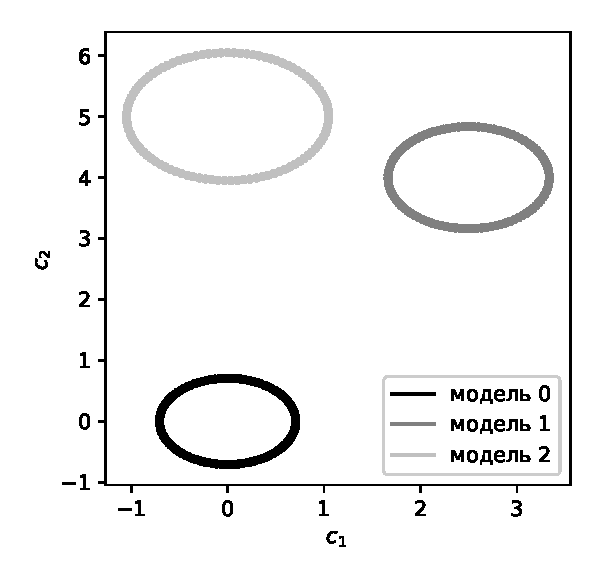
\includegraphics[height = 0.2\textheight]{900.eps}
	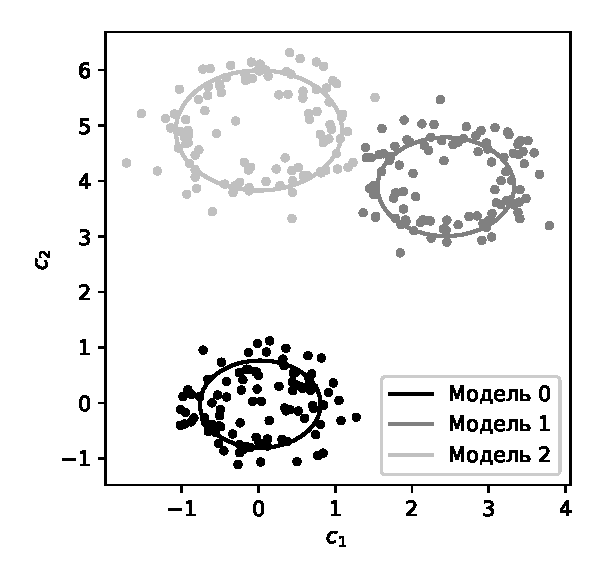
\includegraphics[height = 0.2\textheight]{901.eps}
	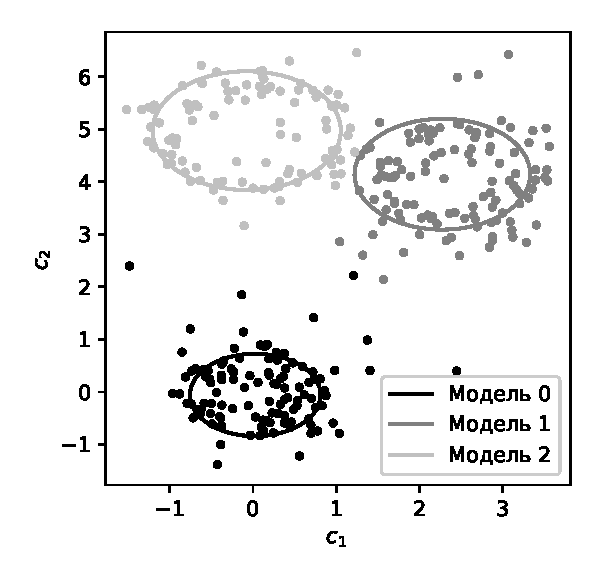
\includegraphics[height = 0.2\textheight]{902.eps}
\caption{Рис.~\ref{ce:fig3}.}
\label{ce:fig3}
\end{figure}

\begin{figure}[h!]
\begin{center}
	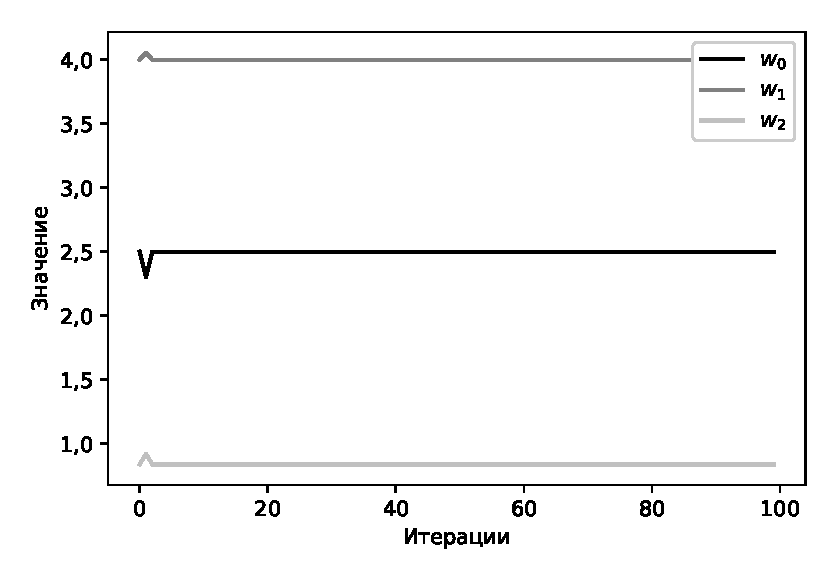
\includegraphics[height = 0.2\textheight]{900noise.eps}
	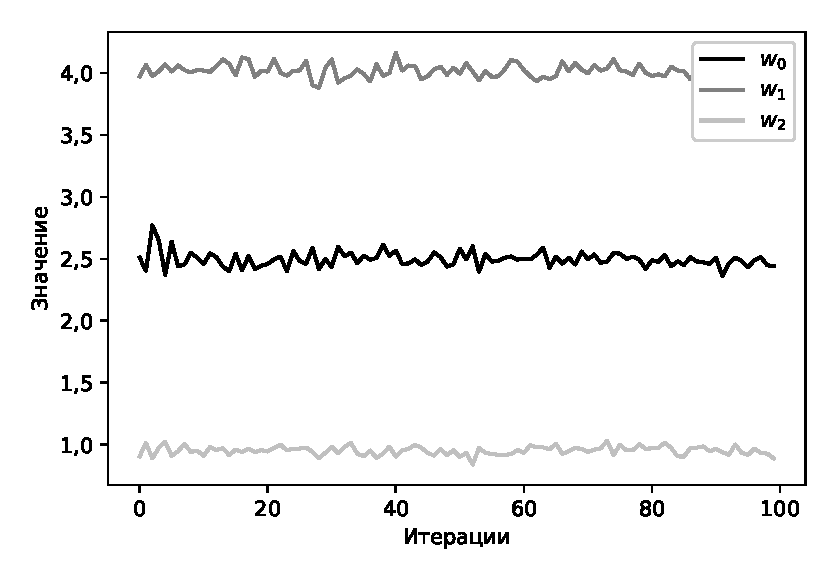
\includegraphics[height = 0.2\textheight]{901noise.eps}\\
	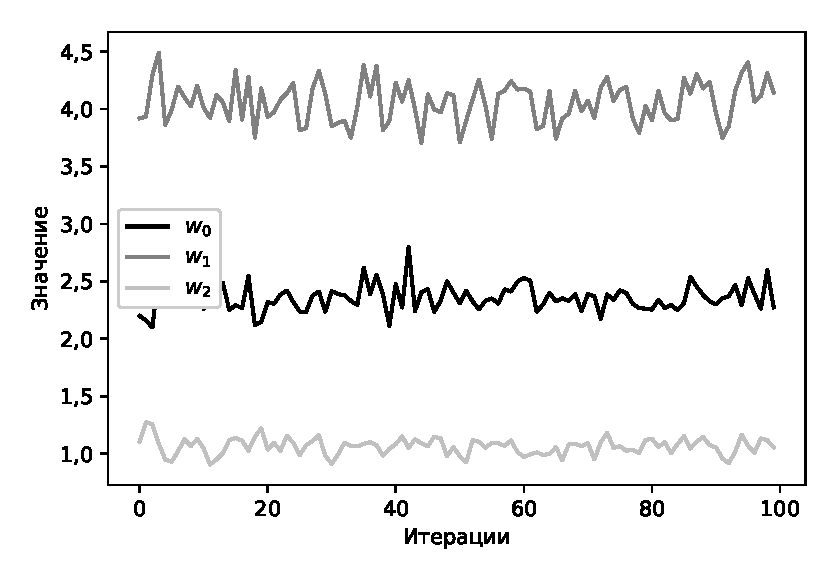
\includegraphics[height = 0.2\textheight]{902noise.eps}
\end{center}
\caption{Рис.~\ref{ce:fig4}.}
\label{ce:fig4}
\end{figure}

\begin{figure}[h!]
\begin{center}
    \includegraphics[width=0.7\textwidth]{3dplot}
\end{center}
\caption{Рис.~\ref{ce:fig5}.}
\label{ce:fig5}
\end{figure}

\begin{figure}[h!]
\begin{center}
    \includegraphics[width=0.8\textwidth]{beta_gamma}
\end{center}
\caption{Рис.~\ref{ce:fig6}.}
\label{ce:fig6}
\end{figure}

\begin{figure}[h!]
\begin{center}
	\includegraphics[height = 0.17\textheight]{not_prior_real_example}
	\includegraphics[height = 0.17\textheight]{prior_real_example}
	\includegraphics[height = 0.17\textheight]{prior_regular_real_example}
\end{center}
\caption{Рис.~\ref{ce:fig6-1}.}
\label{ce:fig6-1}
\end{figure}

\begin{figure}[h!]
\begin{center}
     \includegraphics[width=\textwidth]{experiment_real_not_prior}
\end{center}
     \caption{Рис.~\ref{ce:fig7}.}
    \label{ce:fig7}
\end{figure}

\begin{figure}[h!]
\begin{center}
     \includegraphics[width=\textwidth]{experiment_real_prior}
\end{center}
     \caption{Рис.~\ref{ce:fig8}.}
    \label{ce:fig8}
\end{figure}

\begin{figure}[h!]
\begin{center}
     \includegraphics[width=\textwidth]{experiment_real_regular}
\end{center}
     \caption{Рис.~\ref{ce:fig9}.}
    \label{ce:fig9}
\end{figure}
}

\clearpage
~\\
Рис.~\ref{intro:fig2}. Визуализация экспертной информации в случае с двумя экспертами. Слева направо: экспертная информация первого эксперта; исходные данные; экспертная информация второго эксперта.
~\\
Рис.~\ref{intro:fig1}. Пример изображения радужной оболочки глаза и его контурное представление. Слева: изображение радужной оболочки глаза. Справа: контурное изображение радужной оболочки и аппроксимирующие заданное изображение окружности.
~\\
Рис.~\ref{ce:fig3}. Мультимодель в зависимости от уровня шума в выборке. Слева направо: окружности без шума; шум в радиусе круга; шум в радиусе круга, шум по всему изображению.
~\\
Рис.~\ref{ce:fig4}. Зависимость параметров $r$, $x_0$ и $y_0$ от номера итерации в зависимости от уровня шума в выборке. Слева направо: окружности без шума; шум в радиусе круга; шум в радиусе круга, шум по всему изображению.
~\\
Рис.~\ref{ce:fig5}. Зависимость моделей от уровня шума~$\beta$ в данных, а также от дисперсии априорного распределения~$\gamma$.
~\\
Рис.~\ref{ce:fig6}. Результат аппроксимации данных с разным уровнем шума~$\beta$ и по дисперсии априорного распределения~$\gamma$.
~\\
Рис.~\ref{ce:fig6-1}. Визуализация аппроксимации радужной оболочки. Слева направо: если указан регуляризатор $R_0$; если указан регуляризатор $R_1$; если указан регуляризатор $R_2$.
~\\
Рис.~\ref{ce:fig7}. Визуализация мультимодели в случае регуляризатора~$R_0$.
~\\
Рис.~\ref{ce:fig8}. Визуализация мультимодели в случае регуляризатора~$R_1$.
~\\
Рис.~\ref{ce:fig9}. Визуализация мультимодели в случае регуляризатора~$R_2$.

\end{document}